%\section{课程简介}
\begin{frame}
    \frametitle{课程简介}
    \begin{enumerate}
        \Item 量子光学: is the study of the interaction of individual photons, in the wavelength range from the infrared to the ultraviolet, with ordinary matter - e.g. atoms, molecules, electrons, etc. - described by nonrelativistic quantum mechanics. 
        \Item 课程目标:       
        \begin{itemize}
          \item Grasp of the basic theory of quantum optics
          \item Know of the common application frontiers of quantum optics
      \end{itemize}
    \end{enumerate}
\end{frame}

\begin{frame} 
  \frametitle{分数构成}
      \begin{enumerate}
          \Item Normal results 20\%
          \Item Group discussion 30\%
          \Item Project final report 50\%
      \end{enumerate}
\end{frame}

\begin{frame}
    \frametitle{教材}
      \begin{itemize}
          \Item 《Quantum optics》 Scully, Zubairy, 1997 (Cambridge)        
          \Item 《Quantum Optics: An Introduction》,Fox, Mark,2006
          \Item 《Introductory Quantum Optics》, Gerry, Knight, 2004 (Cambridge)
          \Item 《Statistical Methods in Quantum Optics》Howard, Carmichael, 1999 
          \Item 《Mathematical Methods of Quantum Optics》Ravinder Rupchand Puri, 2001
          \Item 《量子光学研究前沿》上海交通大学出版社出版,张卫平, 2014
          \Item 《量子光学》科学出版社, 郭光灿, 2022
      \end{itemize}
\end{frame}
%%%%%%%%%%%%%%%%%%%%%%%%%%%%%%%%%%%%%

\begin{frame} 
\frametitle{网络教学资源}

牛津大学 Mark Fox (1)
\href{https://www.bilibili.com/video/BV1PK4y1E79Z?t=3.2}{点这里}\\ {\vspace*{2.3em}}

牛津大学 Mark Fox (2)
\href{https://www.bilibili.com/video/BV1mb4y1j7mu/?spm_id_from=autoNext} {点这里} \\ {\vspace*{2.3em}}

慕尼黑大学 Immanuel Bloch
\href{https://www.bilibili.com/video/BV1Ky4y1W7C7?p=1} {点这里}
     
\end{frame}

\begin{frame}
      \frametitle{量子光学相关专业}
      \begin{itemize}
        \Item 光学 (光物理, 光化学, 光材料, 光谱精细结构)
        \Item 光学工程 (激光,光电器件, 光电探测, 非经典光源,量子成像, 量子雷达)  
        \Item 量子信息学 (量子计算, 量子通信, 量子精密测量, 量子传感,  超冷原子)    
    \end{itemize}  
\end{frame}

\begin{frame}
    \frametitle{光学的发展}
    三大光学: 几何光学, 波动光学(物理光学), 量子光学
    \begin{itemize}
        \Item 经典光学(麦克斯韦方程) \\
        不能解释: 黑体辐射, 光电效应, 康普顿效应, 原子光谱, 自发发射, 受激发射...
        \Item 半经典光学(原子能级量子化+经典光场+光子假说)  \\
        不能解释: 延迟选择实验, 量子擦除实验, 相干态, 压缩态, 量子计算, 量子通信, 量子存储...
        \Item 量子光学(量子化粒子+量子化光场)  \\
        解释当前一切光学(实验)现象. 
    \end{itemize}     
\end{frame}

\begin{frame}
    \frametitle{课程内容}
        \begin{enumerate}
            \Item lecture-1   ~~~~半经典光
            \Item lecture-2and3 ~ 量子力学基础与谐振子
            \Item lecture-3and4 ~ 光场量子化
            \Item lecture-6to9  ~~ 相干态与压缩态
            \Item lecture-10to15 ~ 光场测量与光子统计
            \Item lecture-16to20 ~ 光场中的原子
        \end{enumerate}
  \end{frame}

\begin{frame} [plain]
    \frametitle{}
    \Background[1] 
    \begin{center}
    {\huge 第1讲:经典与半经典光学}
    \end{center}  
    \addtocounter{framenumber}{-1}   
\end{frame}
%%%%%%%%%%%%%%%%%%%%%%%%%%%%%%%%%%

\begin{frame}
      \frametitle{本讲要点}
      \begin{enumerate}
        \Item 经典和半经典光学
        \Item 经典和半经典光学主要成就
        \Item 经典和半经典光学所面临的困难
    \end{enumerate}
      
\end{frame}

\section{1. 经典光学}

\begin{frame}
      \frametitle{经典光学的成果:麦克斯韦方程}
    介质中: 定义电位移矢量$\mathbf{D}$ 和磁场强度 $\mathbf{H}$
\[ \mathbf{D}=\epsilon_0 \mathbf{E} + \mathbf{P} = \epsilon_0 \epsilon_r \mathbf{E} \, (*),  \qquad \mathbf{H}=\frac{1}{\mu_0} \mathbf{B} -\mathbf{M}= \frac{1}{\mu_0\mu_r}\mathbf{B} \, (*)\]
麦克斯韦方程:

\[ \begin{aligned}
        \text{I}~~~ \hspace*{2em}&\nabla \cdot \mathbf{D} =\rho _f  \\  
        \text{II}~~ \hspace*{2em}&\nabla \cdot \mathbf{B} = 0  \\  
        \text{III}~ \hspace*{2em}&\nabla \times  \mathbf{E} = -\cfrac{\partial \mathbf{B}}{\partial t }  \\  
        \text{IV~}~ \hspace*{2em}&\nabla \times  \mathbf{H} = \mathbf{J}_f +  \cfrac{\partial \mathbf{D}}{\partial t } 
    \end{aligned} \]
\end{frame}

\begin{frame}
      \frametitle{电磁波}
    对于真空 ($\rho _f =0, \mathbf{J}_f =0 $),  \[ \mathbf{B} = \mu_0 \mathbf{H}, \qquad  \mathbf{D} = \epsilon_0 \mathbf{E} \]
代入麦克斯韦方程(IV)
 \[ \nabla \times  \mathbf{H} = \mathbf{J}_f +  \cfrac{\partial \mathbf{D}}{\partial t } \]
得: \[ \nabla \times \mathbf{B} = \mu_0\epsilon_0 \cfrac{\partial \mathbf{E}} {\partial t } \]
由麦克斯韦方程(III)
\[    
\begin{aligned}
  \nabla \times (\nabla \times  \mathbf{E}) &= - \nabla \times \cfrac{\partial \mathbf{B}}{\partial t } \\
  &= - \mu_0\epsilon_0  \cfrac{\partial ^2 \mathbf{E}} {\partial t^2 }
\end{aligned} \]  
\end{frame}

\begin{frame}
      \frametitle{}
    由于
  \[
  \begin{aligned}
      \nabla \times (\nabla \times  \mathbf{E}) &=  \nabla (\nabla \cdot  \mathbf{E})- \nabla^2 \mathbf{E} \\
      &= - \nabla^2 \mathbf{E} 
  \end{aligned} \]
  得:
  \[
  \nabla^2 \mathbf{E}= \mu_0\epsilon_0 \cfrac{\partial ^2 \mathbf{E}} {\partial t^2 }\]
  由于$ c= \frac{1}{\sqrt{\mu_0\epsilon_0}} $, 方程可写为
  \[\boxed{\mathbf{E}_{tt} =c^2\nabla^2 \mathbf{E}}\]
  ~~\\
  这是波动方程标准型(见数理方程), 这表明光波就是电磁波 \\ 若给出定解条件, 方程可求解 \\  
\end{frame}

\begin{frame}
 \frametitle{}
 \[\mathbf{E}_{tt} =c^2\nabla^2 \mathbf{E}\]
 这是矢量方程. 描述光的偏振. 
   \begin{center}
        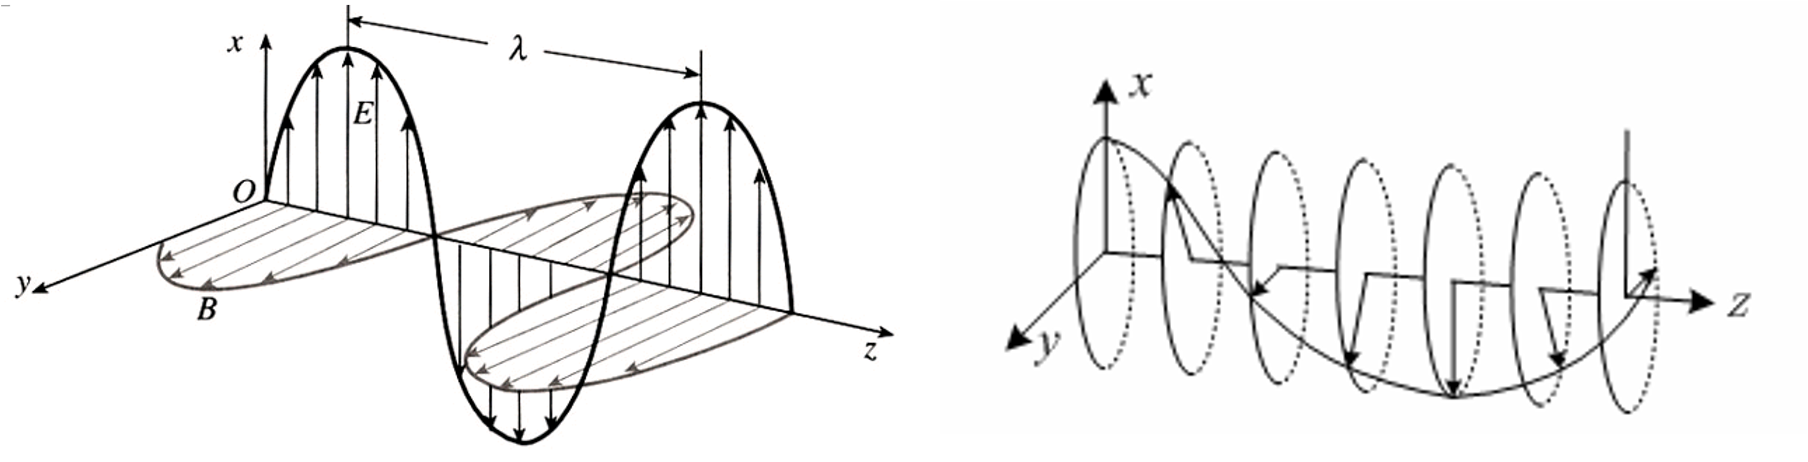
\includegraphics[width=0.8\textwidth]{figs/10.png}
   \end{center}
 考虑标量化.
 \begin{enumerate}
     \item 线偏振 $\mathbf{E}(z,t) = E_x(z,t) \hat{e}_x $ 
     \item 圆偏振 $\mathbf{E}(z,t) = E_x(z,t) \hat{e}_{\sigma}, \qquad \text{with} \qquad \hat{e}_{\pm}= \mp \frac{1}{\sqrt{2}} (\hat{x} \pm \hat{y}) $
 \end{enumerate}
\end{frame}

\begin{frame}
      \frametitle{}
      ~~\\
    \例 [1. 试求一维光学腔中的线偏振电磁场] {
      \begin{center}
           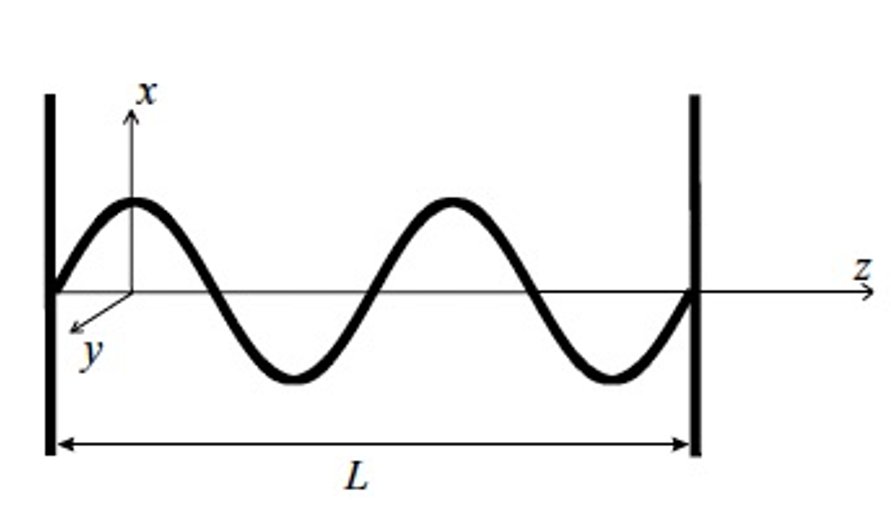
\includegraphics[width=0.4\textwidth]{figs/1.png}
      \end{center}  
      光学腔: $0\leq z\leq L$ \\  
      边界条件: $E_x(0)=E_x(L)=0$  
    }
    \解  设 $\displaystyle  E_x(z,t)=T(t)Z(z) $,代入波动方程 
    \[\mathbf{E}_{tt} =c^2\nabla^2 \mathbf{E}\]
\end{frame}

\begin{frame}
      \frametitle{} 
    得:
	\begin{equation*}
		 T~^{''}(t)Z(z) =c~^2 T(t)Z~^{''}(z) 
	\end{equation*}
	分离变量, 令: {\hspace*{2em}}
      $$ \dfrac{T~^{''}}{c~^2 T}=\dfrac{Z~^{''} }{Z} =-\lambda $$ \\ \vspace{0.3cm}
    转化为两常微分方程 \\ \vspace{0.3cm}
    方程(I):
      $\displaystyle  \begin{cases}
          Z~^{''} +\lambda Z=0  ~~,~~ 0<z<L\\
          Z(0)=0 ~,~Z(L)=0
      \end{cases}$ \\	
    方程(II):
      $\displaystyle  \begin{cases}
          T~^{''} +\lambda {c~^2 T}=0 \\
          ......
      \end{cases}$ \\	  
\end{frame}

\begin{frame}
      \frametitle{}
    特征(辅助)方程法解方程(I)  
    \begin{enumerate}
    \IItem 固有值:$\displaystyle  \lambda_n=\frac{n^2\pi^2}{L^2}= \omega^2 _n, \quad k_n=\frac{\omega_n}{c} $ 
    \IItem 固有解:$\displaystyle  E_n(z)=\sin (\omega_n z) $
    \end{enumerate}
    解方程II : 	\[ T~^{''} +\lambda {c~^2 T}=0 \] \\ 
	代入$\lambda_n$, 得:
	$\displaystyle  T~^{''} +\lambda~_n c~^2 ~T=0 $ \\
	变形为:\[  T~^{''} +\omega ~_n ^2 {c~^2 T}=0 \]
	特征方程有虚根,通解 :\\
	\hspace{3cm}	$\displaystyle 	T~_n=c~_n\cos \omega_n~c~t+ d~_n\sin \omega ~_n~c~t $  \\ \vspace{1em}
\end{frame}

\begin{frame}
    \frametitle{} 
    ~\\
    原方程的基本解:\\ {\vspace*{0.3em}}
	$\begin{array}{llll}
		E_n (z,t) &=& T_n(t)Z_n(z)\\
		&=& (c_n\cos \omega_nct+ d_n\sin \omega _nct ) \sin \omega_n z\\
        &=&a_n \exp(i \omega_n ct) \sin \frac{ n\pi z}{L} \\
	\end{array}$ \\  {\vspace*{0.6em}}    
    \begin{enumerate}
    %\IItem 基本解:$\displaystyle E_{n}(z,t) = a_n q_n (t) \sin (k_n z), \quad \text{with} \quad a_n = \left( \frac{2 \omega ^2}{V \epsilon_0}\right)^{1/2} $
    \IItem 基本解:$\displaystyle E_{n}(z,t) = a_n q_n (t) \sin (k_n z) $
    \IItem 叠加解:$\displaystyle E_{x}(z,t) = \sum\limits_{n=1}^{\infty } a_n q_n (t) \sin (k_n z)$
    \end{enumerate}	
    把解代回由麦克斯韦方程(III), 得磁场叠加解 \\ 
    \[ H_{y}(z,t) = \sum\limits_{n=1}^{\infty } a_n \frac{\epsilon_0}{k_n}q_n ' (t) \cos (k_n z)\] 
\end{frame}

\begin{frame}
      \frametitle{}
    令: 
    \[  L \to \infty \]
    得自由场解 
    \[  E_{x}(z,t) = \frac{1}{2} E_{0x}(z) \exp [i(kz-\omega t)] \]
    ~~\\ 
    电磁场的哈密顿(能量)
    \[ H = \frac{1}{2} \int_V d V \left[ \epsilon_0 \mathbf{E^2}(\mathbf{r},t) + \frac{1}{\mu_0}\mathbf{B^2}(\mathbf{r},t)\right]\]
\end{frame}

\begin{frame} 
\frametitle{波动光学基本结论}
    电磁场是一系列基本振动模式的叠加.\\ 
    \[ E_{x}(z,t) = \sum\limits_{n=1}^{\infty } a_n q_n (t) \sin (k_n z)\]
    \[ H_{y}(z,t) = \sum\limits_{n=1}^{\infty } a_n \frac{\epsilon_0}{k_n}q_n ' (t) \cos (k_n z)\] 
    自由场是自由振动;存在电荷或电流等环境,则是受迫振动, 波动方程为:
    \[\mathbf{E}_{tt} -c^2\nabla^2 \mathbf{E} = \mu_0 \frac{\partial ^2 \mathbf{P}  }{\partial t^2}\]  
\end{frame}

\begin{frame}
      \frametitle{经典光学面临的困难}
      基于麦克斯韦方程的波动光学, 不能解释如下实验
      \begin{itemize}
          \item 黑体辐射, 
          \item 光电效应, 
          \item 康普顿效应, 
          \item 原子光谱, 
          \item 光的发射与吸收...
      \end{itemize}
      * 对上述问题的解释导致量子力学的建立
\end{frame}

\section{2. 半经典光学}

\begin{frame}
      \frametitle{光量子假说}
      1900年, 普朗克提出热辐射能量子假说
      \[E= n \varepsilon , \qquad \varepsilon= h \nu= \hbar \omega\]
      1905年,爱因斯坦提出光量子假说, 揭示光的波粒二象性本质.  \\ {\vspace*{1em}}
      \[E= h \nu= \hbar \omega, \qquad  \mathbf{p}=\frac{h}{\lambda} \mathbf{n} = \hbar \mathbf{k} \]  
      \\  \vspace*{3em}

      基此发展出半经典光学, 可成功解释经典光学所面临的上述困难!
\end{frame}

\begin{frame}
    \frametitle{半经典光学}     
    \begin{itemize}
        \Item 量子化原子能级
        \Item 经典的光学场+光量子假说
    \end{itemize}  
\end{frame}

\begin{frame}
      \frametitle{}
      \例 [2. 试采用半经典方法处理光与原子的相互作用问题] {}
      \解~ 考虑沿z轴传播的单色光 
      \[ \left\{\begin{array}{l}
        E_{x}=E_{0} \cos \left(\frac{2 \pi}{\lambda} z-\omega t\right) \\
        E_{y}=E_{z}=0
        \end{array}\right. \]
     光与原子的相互作用发生在原子内部, 这个尺度的光场可认为是均匀场
     \[E_{x}=E_{0} \cos \left(\omega t\right)  \]
     光波所产生的能量可看做是对原子能级的微扰 
     \[\begin{aligned}
        &\hat{H}^{\prime}=e\mathbf{r}\cdot\mathbf{E}  = ex E_{x} \\
        &=\frac{1}{2} \operatorname{ex} E_{0}\left[e^{i \omega t}+e^{-i \omega t}\right] \\
        &=\hat{F}\left[e^{i \omega t}+e^{-i \omega t}\right]
        \end{aligned}
      \]
\end{frame}

\begin{frame}
      \frametitle{}
      代入含时微扰公式
      \[ \omega_{m \rightarrow k}=\frac{2 \pi}{\hbar}\left|F_{k m}\right|^{2} \delta\left(\varepsilon_{k}-\varepsilon_{m}+\hbar \omega\right) \]
      对于自然光,可得跃迁概率:
      \[ w_{k \rightarrow m}=\frac{4 \pi^{2} e^{2}}{3 \hbar^{2}} I\left(\omega_{m k}\right)\left|\vec{r}_{m k}\right|^{2} = B_{km} I\left(\omega_{m k}\right)\]
      求得爱因斯坦吸收系数 $B_{km}$ \\ 
      同理,得爱因斯坦受激发射系数 $B_{mk}$  \\ 
      代入电磁辐射平衡条件(发射的光子数等于吸收的光子数) 
      \[N_{m}\left[A_{m k}+B_{m k} I\left(\omega_{m k}\right)\right]=N_{k} B_{k m} I\left(\omega_{m k}\right) \]
      得自发发射系数 $A_{mk}$ 
\end{frame}

\begin{frame}
      \frametitle{}
      基于光子数目决定电磁场强度的基本假设, 得辐射场强度
    \[\begin{aligned}
        J_{m k} &=N_{m} A_{m k} \hbar \omega_{m k} \\
        &=N_{m} \frac{4 e^{2} \omega_{m k}^{4}}{3 c^{3}}\left|\vec{r}_{k m}\right|^{2} 
        \end{aligned} \] {\vspace*{2.3em}}
    成功解决辐射场问题, 如: 选择定则, 激发态寿命, 常见光谱, ... \\ \vspace*{2.0em}
    增加自旋, 解决光谱分裂问题 \\
    增加旋-轨耦合,解决复杂光谱问题 \\ 
    增加非线性效应,解决变频问题 \\
\end{frame}

\begin{frame}
    \frametitle{半经典光学面临的困难}
    半经典半量子光学取得了具大成功. \\ 
    但不能解释如下光学现象
    \begin{itemize}
        \item 延迟选择实验
        \item 量子擦除实验
        \item 相干态
        \item 压缩态
        \item 纠缠光子对
        \item 单光子源
        \item 量子隐形传态
    \end{itemize}
    * 这些问题的解释导致第二次量子革命, 1956年后, 发展出非经典光源 (激光, 压缩光, 单光子), 人类进入量子光学时代.
\end{frame}

\begin{frame}
    \frametitle{惠勒延迟选择实验}
    \begin{center}
        \includegraphics[width=0.6\textwidth]{figs/choose.png} \\
    \end{center} 
    {\Bullet} 光子总是处于叠加
    {\Bullet} 光路的说法是不成立的
\end{frame}

%\begin{frame}
%    \frametitle{量子擦除实验}
%    \begin{center}
%        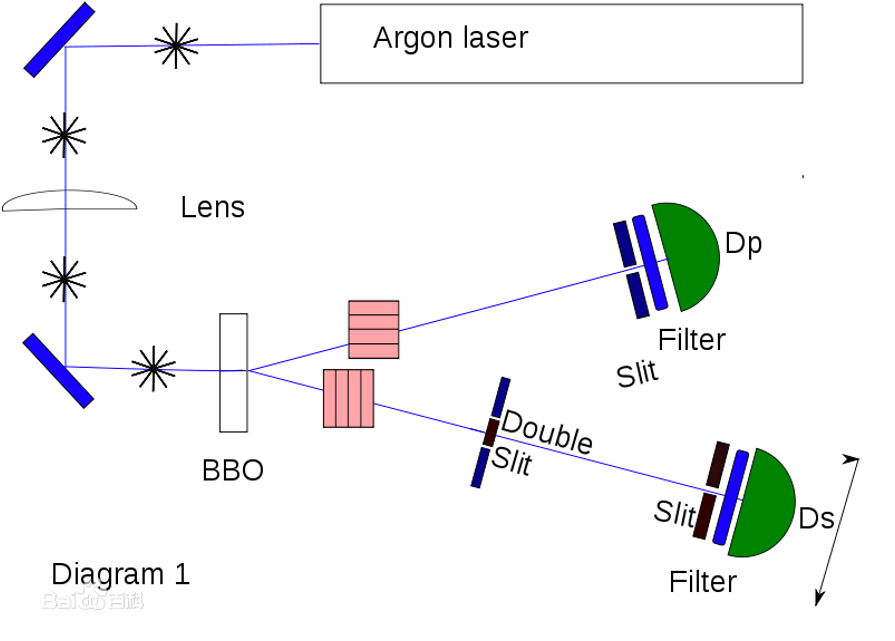
\includegraphics[width=0.6\textwidth]{figs/c1.%png} \\
%    \end{center} 
%\end{frame}
%
%\begin{frame}
%    \frametitle{}
%    \begin{center}
%        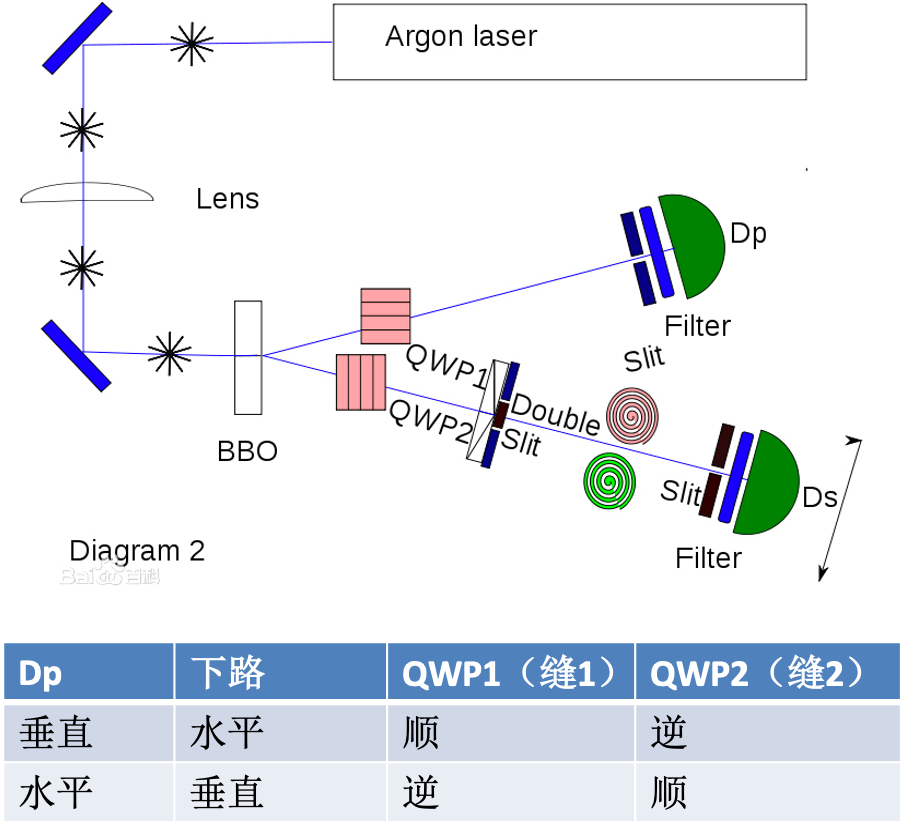
\includegraphics[width=0.6\textwidth]{figs/c2.%png} \\
%    \end{center} 
%\end{frame}
%
%\begin{frame}
%    \frametitle{}
%    \begin{center}
%        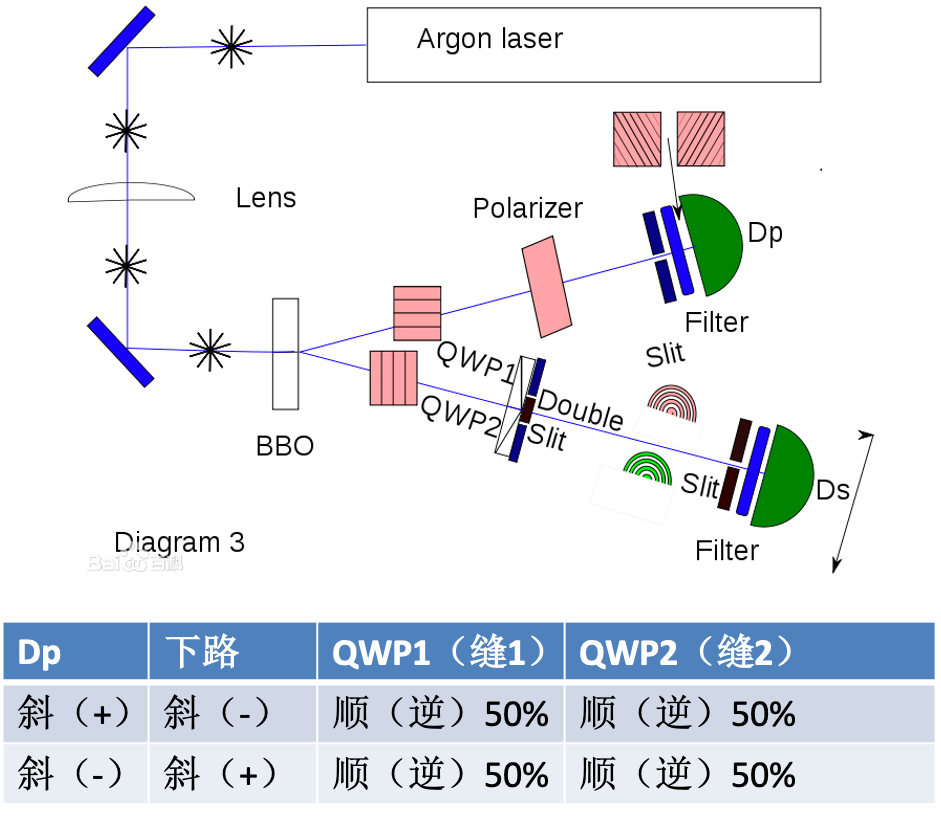
\includegraphics[width=0.6\textwidth]{figs/c3.%png} \\
%    \end{center} 
%\end{frame}

%%%%%%%%%%%%%%%%%%%%%%%%%%%%%%%%%%%%%%%%%%%%%%%%%%%%%%%%%%%%%%%%%%%
\begin{frame}
    \frametitle{课外作业}
    \begin{enumerate}
        \item 补全例1的计算
        \item 补全例2的计算
        \item 了解非线性光学
        \item 量子擦除实验说明什么?
    \end{enumerate}
\end{frame}
%%%%%%%%%%%%%%%%%%%%%%%%%%%%%%%%%%%%%%%%%%%%%%%%%%%%%%%%%%%%%%%%%%%

